\section{Results}
\label{sec:results}
\subsection{Discrimination of separately evaluated fold models}
All 15 principal-model runs and five supplementary mean-pooling runs completed training and formal evaluation. Twenty evaluation receipts and 60 registered report identities were verified. Each seed-44 fold model was evaluated separately on the same 175 holdout patients, including 56 positive outcomes. Table~\ref{tab:main} reports the mean and sample standard deviation of the five fold-specific metrics. Macro is first computed within each fold and then averaged across folds; no model probabilities are averaged.
\begin{table*}[t]
\centering
\small
\caption{Performance on the same fixed internal holdout (175 patients, 56 pCR positive). Entries are mean $\pm$ sample SD of metrics computed separately for the five seed44 fold models. Probabilities are not averaged. Macro first averages T0--T2 metrics within each fold. F1 uses threshold 0.5. Fold SD is descriptive; the five models share the holdout and overlapping training sets. Paired Macro differences are in Table~\ref{tab:bootstrap}.}
\label{tab:main}
\begin{tabular}{llrrr}
\toprule
Model & Landmark & AUROC & AP & F1 \\
\midrule
NoJEPA & T0 & 0.7209 $\pm$ 0.0117 & 0.5749 $\pm$ 0.0295 & 0.5441 $\pm$ 0.0378 \\
NoJEPA & T1 & 0.7219 $\pm$ 0.0113 & 0.5815 $\pm$ 0.0185 & 0.5458 $\pm$ 0.0408 \\
NoJEPA & T2 & 0.7230 $\pm$ 0.0112 & 0.5812 $\pm$ 0.0145 & 0.5411 $\pm$ 0.0409 \\
NoJEPA & Macro & 0.7219 $\pm$ 0.0113 & 0.5792 $\pm$ 0.0202 & 0.5437 $\pm$ 0.0383 \\
DirectReadout & T0 & 0.7304 $\pm$ 0.0135 & 0.5854 $\pm$ 0.0200 & 0.5447 $\pm$ 0.0302 \\
DirectReadout & T1 & 0.7306 $\pm$ 0.0120 & 0.5891 $\pm$ 0.0226 & 0.5485 $\pm$ 0.0178 \\
DirectReadout & T2 & 0.7299 $\pm$ 0.0116 & 0.5920 $\pm$ 0.0228 & 0.5685 $\pm$ 0.0329 \\
DirectReadout & Macro & 0.7303 $\pm$ 0.0124 & 0.5888 $\pm$ 0.0214 & 0.5539 $\pm$ 0.0233 \\
ForecastAttention & T0 & 0.7294 $\pm$ 0.0171 & 0.5924 $\pm$ 0.0124 & 0.5334 $\pm$ 0.0350 \\
ForecastAttention & T1 & 0.7381 $\pm$ 0.0161 & 0.6012 $\pm$ 0.0156 & 0.5563 $\pm$ 0.0330 \\
ForecastAttention & T2 & 0.7421 $\pm$ 0.0167 & 0.6033 $\pm$ 0.0191 & 0.5510 $\pm$ 0.0427 \\
ForecastAttention & Macro & 0.7365 $\pm$ 0.0159 & 0.5990 $\pm$ 0.0151 & 0.5469 $\pm$ 0.0334 \\
\bottomrule
\end{tabular}
\end{table*}


\fullmodel{} had fold-mean T0/T1/T2 AUROCs of 0.7294/0.7381/0.7421 and AP values of 0.5924/0.6012/0.6033 (Fig.~\ref{fig:discrimination}). Its Macro AUROC/AP/F1 was 0.7365/0.5990/0.5469, with fold standard deviations of 0.0159/0.0151/0.0334. Corresponding mean Macro values were 0.7219/0.5792/0.5437 for \nojepa{} and 0.7303/0.5888/0.5539 for \direct{}. Forecast attention had the highest mean Macro AUROC and AP, while direct readout had the highest mean Macro F1 among all four variants. At T0, forecast attention's mean AUROC was slightly below direct readout (0.7294 versus 0.7304), whereas it was higher at T1 and T2. The discrimination ordering was therefore not uniform across landmarks.

\begin{figure*}[t]
\centering
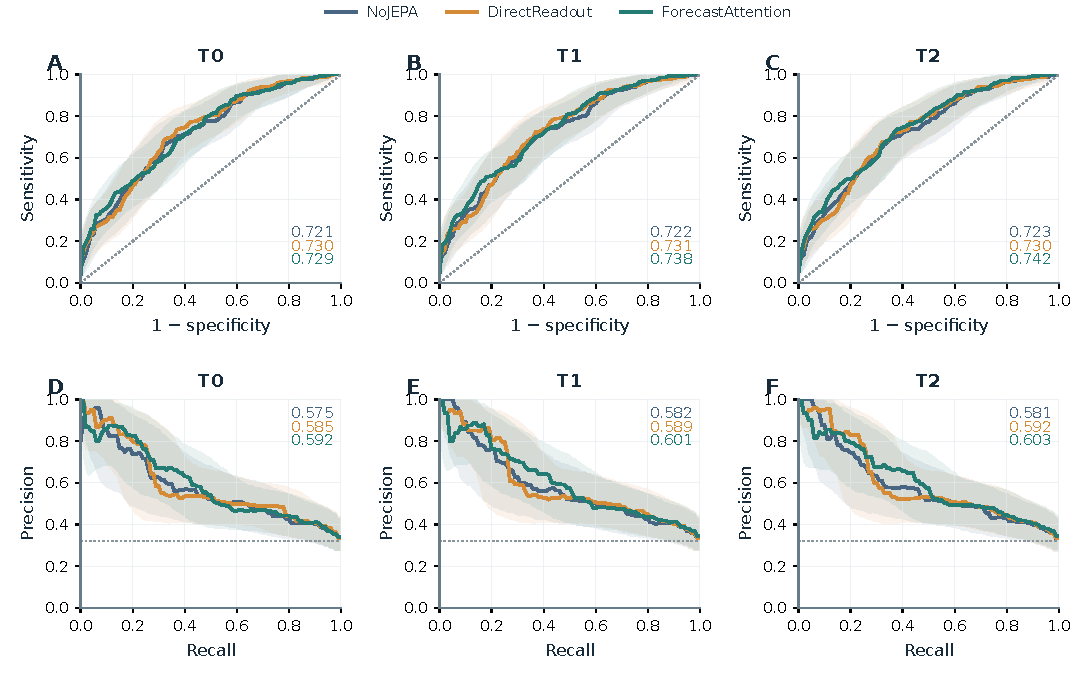
\includegraphics[width=\textwidth]{figures/discrimination.pdf}
\caption{Discrimination of seed-44 fold models evaluated separately. (A--C) Mean ROC curves; (D--F) mean precision--recall curves. Curves are computed per fold, interpolated onto a common grid, and averaged across five folds. Shading gives conditional 95\% shared-patient-bootstrap intervals for the mean curve. Colored values summarize directly calculated per-fold AUROC or non-interpolated AP, whose means need not equal the area under the displayed mean curve. The dotted PR reference is the 0.32 positive prevalence. No probabilities are averaged between fold models.}
\label{fig:discrimination}
\end{figure*}

Under direct readout, adding future-state supervision increased mean Macro AUROC/AP/F1 by +0.0084/+0.0097/+0.0102. The full forecast-attention model gave further mean AUROC and AP increases of +0.0062 and +0.0101 relative to \direct{}, but mean F1 decreased by 0.0070. The first comparison more closely isolates auxiliary supervision, whereas the second also changes forecast inputs, pooling, and classifier width. Direct readout had higher Macro AUROC than \nojepa{} in all five folds. Forecast attention exceeded both direct controls in four folds but was lower in fold 5: its Macro AUROC was 0.7170, compared with 0.7347 for \nojepa{} and 0.7477 for \direct{}. All fold-specific results are retained in Tables~\ref{tab:foldresults} and~\ref{tab:foldresults_forecast}.

The supplementary \meanmodel{} had mean Macro AUROC/AP/F1 of 0.7348/0.5845/0.5458 (Table~\ref{tab:pooling}). Forecast attention's corresponding differences were +0.0017/+0.0144/+0.0011, but all paired intervals included zero. Mean pooling had slightly higher T0 AUROC than forecast attention (0.7317 versus 0.7294). The mean estimates do not establish a consistent attention benefit across folds, landmarks, and metrics.

The paired patient intervals for every principal Macro AUROC/AP/F1 comparison included zero (Fig.~\ref{fig:paired}). The full-versus-\nojepa{} AUROC difference was +0.0146 [$-0.0073$, 0.0376], the \direct{}--\nojepa{} difference +0.0084 [$-0.0049$, 0.0212], and the full-versus-direct difference +0.0062 [$-0.0136$, 0.0275]. The full-versus-direct F1 difference was $-0.0070$ [$-0.0398$, 0.0242]. These conditional patient intervals are distinct from descriptive fold standard deviations and exclude retraining and seed-selection uncertainty.
None of the nine principal Macro comparisons met the 0.05 criterion, and all nine had within-family Holm-adjusted $p=1.0000$ (Table~\ref{tab:bootstrap}). For example, the full-versus-\nojepa{} Macro AUROC difference had raw $p=0.19246$, and the full-versus-direct comparison had raw $p=0.54536$. These results do not establish superiority or equivalence; they qualify the descriptive ranking differences conditional on the selected seed and fitted models.
\begin{table*}[t]
\centering
\small
\caption{Exploratory principal Macro comparisons. All metrics use approximate, null-centered paired patient-bootstrap tests with 99,999 shared resamples. Within each draw, metrics are computed for each fold model then equally averaged; probabilities are never averaged. All $p$ values are two-sided. Holm$_9$ adjusts the nine entries here; Holm$_{90}$ is the sensitivity analysis over all principal and secondary tests. Sig. refers to Holm$_9$. Direct and Attention abbreviate DirectReadout and ForecastAttention. $^{*}p_{\mathrm{Holm}}<0.05$, $^{**}p_{\mathrm{Holm}}<0.01$, $^{***}p_{\mathrm{Holm}}<0.001$; ns, not significant after the stated correction. Intervals are unadjusted 95\% patient-bootstrap intervals (2,000 shared draws) and need not agree with adjusted test decisions. All analyses condition on the five fixed seed44 fold models; folds are not resampled and share one holdout.}
\label{tab:bootstrap}
\begin{tabular}{llrrrrc}
\toprule
Comparison & Metric & Difference [95\% CI] & $p$ & $p_{\mathrm{Holm},9}$ & $p_{\mathrm{Holm},90}$ & Sig. \\
\midrule
Direct -- NoJEPA & AUROC & +0.0084 [-0.0049, +0.0212] & 0.2199 & 1.0000 & 1.0000 & ns \\
Direct -- NoJEPA & AP & +0.0097 [-0.0129, +0.0297] & 0.3731 & 1.0000 & 1.0000 & ns \\
Direct -- NoJEPA & F1 & +0.0102 [-0.0118, +0.0323] & 0.3595 & 1.0000 & 1.0000 & ns \\
Attention -- NoJEPA & AUROC & +0.0146 [-0.0073, +0.0376] & 0.1925 & 1.0000 & 1.0000 & ns \\
Attention -- NoJEPA & AP & +0.0198 [-0.0158, +0.0621] & 0.3060 & 1.0000 & 1.0000 & ns \\
Attention -- NoJEPA & F1 & +0.0032 [-0.0339, +0.0379] & 0.8616 & 1.0000 & 1.0000 & ns \\
Attention -- Direct & AUROC & +0.0062 [-0.0136, +0.0275] & 0.5454 & 1.0000 & 1.0000 & ns \\
Attention -- Direct & AP & +0.0101 [-0.0239, +0.0518] & 0.5816 & 1.0000 & 1.0000 & ns \\
Attention -- Direct & F1 & -0.0070 [-0.0398, +0.0242] & 0.6600 & 1.0000 & 1.0000 & ns \\
\bottomrule
\end{tabular}
\end{table*}


\begin{figure*}[t]
\centering
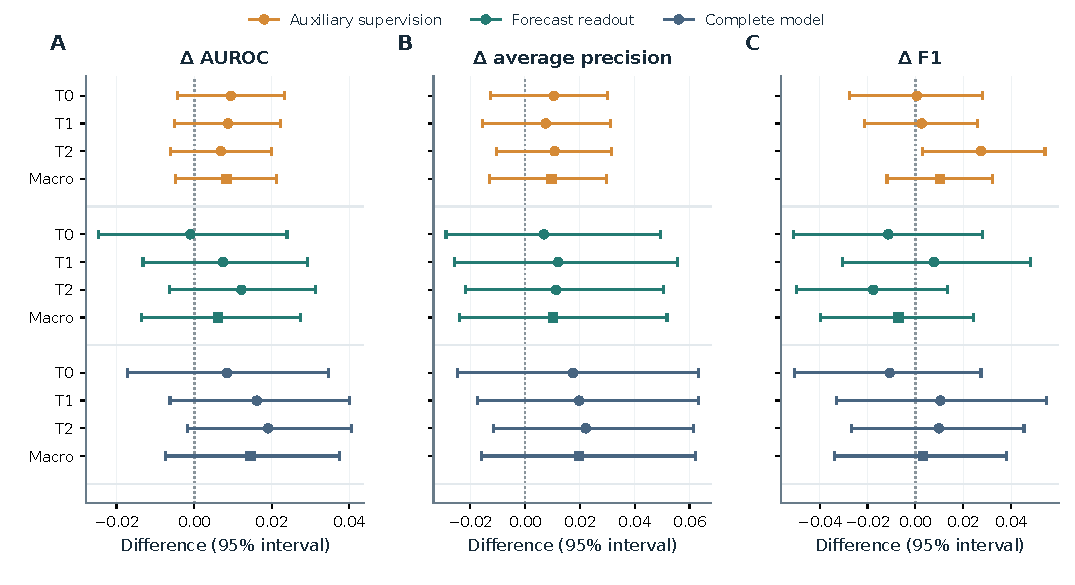
\includegraphics[width=\textwidth]{figures/paired_comparisons.pdf}
\caption{Paired differences in fold-mean metrics at T0, T1, T2, and Macro. Colors distinguish auxiliary supervision, additional forecast readout, and the complete-model contrast. Squares denote Macro estimates. Bars are unadjusted 95\% patient-bootstrap intervals, with every patient draw shared across folds, models, and landmarks. Metrics are computed separately within folds before averaging. Adjusted tests appear in Tables~\ref{tab:bootstrap} and~\ref{tab:significance_landmarks}. The five fold models do not create independent test cohorts.}
\label{fig:paired}
\end{figure*}

\subsection{Threshold behavior and class imbalance}
\begin{table*}[t]
\centering
\small
\caption{Operating characteristics at threshold 0.5. Entries average metrics computed separately for five seed44 fold models; Macro first averages T0--T2 within each fold. No probabilities are averaged. The same 175 patients appear in every evaluation.}
\label{tab:extended_operating}
\begin{tabular}{llrrrrrr}
\toprule
Model & Landmark & Sens. & Spec. & PPV & NPV & BA & MCC \\
\midrule
NoJEPA & T0 & 0.614 & 0.701 & 0.491 & 0.796 & 0.658 & 0.301 \\
NoJEPA & T1 & 0.614 & 0.703 & 0.492 & 0.796 & 0.658 & 0.302 \\
NoJEPA & T2 & 0.600 & 0.711 & 0.494 & 0.791 & 0.655 & 0.298 \\
NoJEPA & Macro & 0.610 & 0.705 & 0.492 & 0.794 & 0.657 & 0.300 \\
\midrule
DirectReadout & T0 & 0.625 & 0.686 & 0.485 & 0.796 & 0.655 & 0.296 \\
DirectReadout & T1 & 0.625 & 0.692 & 0.492 & 0.798 & 0.659 & 0.303 \\
DirectReadout & T2 & 0.657 & 0.694 & 0.504 & 0.813 & 0.676 & 0.334 \\
DirectReadout & Macro & 0.636 & 0.691 & 0.494 & 0.802 & 0.663 & 0.311 \\
\midrule
ForecastAttention & T0 & 0.646 & 0.642 & 0.473 & 0.809 & 0.644 & 0.285 \\
ForecastAttention & T1 & 0.750 & 0.556 & 0.455 & 0.836 & 0.653 & 0.298 \\
ForecastAttention & T2 & 0.714 & 0.583 & 0.465 & 0.836 & 0.649 & 0.297 \\
ForecastAttention & Macro & 0.704 & 0.594 & 0.464 & 0.827 & 0.649 & 0.293 \\
\bottomrule
\end{tabular}
\end{table*}

At threshold 0.5, mean Macro sensitivity/NPV was 0.7036/0.8269 for \fullmodel{}, compared with 0.6357/0.8023 for \direct{}. Higher sensitivity accompanied lower specificity (0.5938 versus 0.6908) and PPV (0.4643 versus 0.4938). The paired sensitivity difference was +0.0679 [0.0262, 0.1103], while the specificity difference was $-0.0969$ [$-0.1280$, $-0.0685$]. These operating-point differences should accompany the ranking means. The full-versus-direct specificity decrease met both the secondary-family and all-90 Holm criteria (adjusted $p=0.00081$ and 0.00090). Relative to \nojepa{}, forecast attention had a mean sensitivity increase of +0.0940 and specificity decrease of 0.1109; their secondary-family adjusted values were 0.03002 and 0.00081, respectively, and their all-90 values were 0.03344 and 0.00090. These three operating-point comparisons were the only secondary tests meeting the family-adjusted criterion. The two specificity tests reached the raw Monte Carlo resolution of $10^{-5}$, rather than a zero $p$ value.

The full model's fold-mean true-positive counts at T0/T1/T2 were 36.2/42.0/40.0, with false-positive counts 42.6/52.8/49.6. These are averages of integer counts from five correlated predictors, not fractional patients or a combined confusion matrix. At T1, sensitivity rose to 0.75 while specificity fell to 0.5563. Its F1 was 0.5334/0.5563/0.5510 across T0/T1/T2, exceeding direct readout only at T1. Improved ranking and a fixed-threshold decision rule therefore gave different patterns.

Among the principal variants, \direct{} had the highest mean Macro balanced accuracy (0.6632) and MCC (0.3109), compared with 0.6571/0.3000 for \nojepa{} and 0.6487/0.2931 for \fullmodel{}. Mean Macro accuracy was 0.6731, 0.6743, and 0.6290, respectively. All were below the all-negative accuracy reference of 0.68, although direct readout's T2 accuracy was 0.6823. The supplementary \meanmodel{} had Macro balanced accuracy 0.6529, MCC 0.2990, and accuracy 0.6450. Accuracy alone would obscure the minority-class behavior.

Fold-specific validation Youden thresholds changed mean holdout Macro F1 from 0.5437 to 0.5515 for \nojepa{}, 0.5539 to 0.5372 for \direct{}, 0.5469 to 0.5411 for \fullmodel{}, and 0.5458 to 0.5236 for \meanmodel{} (Table~\ref{tab:extended_threshold}). For forecast attention, mean sensitivity decreased to 0.6440 while specificity increased to 0.6560. Thus the validation-selected thresholds did not consistently improve F1. The thresholds were fitted separately on the matching model's validation predictions and then applied to that model's test predictions; no test outcome selected a threshold. Reuse of validation patients for checkpoint selection limits this analysis to a sensitivity check.

\subsection{Longitudinal information and probability quality}
The paired fold-mean T2--T0 AUROC change was +0.0127 [0.0026, 0.0235] for \fullmodel{}, +0.0021 [$-0.0027$, 0.0073] for \nojepa{}, and $-0.0005$ [$-0.0086$, 0.0081] for \direct{}. Forecast attention's corresponding AP change was +0.0110 [$-0.0048$, 0.0264] and F1 change +0.0176 [$-0.0051$, 0.0424]. Its AUROC interval excluded zero without multiplicity correction, whereas the AP and F1 intervals did not. The AUROC change had raw $p=0.01892$ but secondary-family and all-90 Holm $p=1.0000$; it therefore did not meet the adjusted criterion. Outcome-conditioned probability-change distributions in Fig.~\ref{fig:scorechanges} retain the separate fold predictions.

\begin{table*}[t]
\centering
\small
\caption{Probability quality: five-fold metric mean $\pm$ sample fold SD for seed44. Metrics are computed separately from each model score vector; Macro averages T0--T2 within fold. Lower is better; ECE uses ten equal-width bins.}
\label{tab:calibration}
\begin{tabular}{lrrr}
\toprule
Model & NLL & Brier & ECE \\
\midrule
NoJEPA & 0.5974 $\pm$ 0.0111 & 0.2069 $\pm$ 0.0045 & 0.1310 $\pm$ 0.0119 \\
DirectReadout & 0.5995 $\pm$ 0.0228 & 0.2073 $\pm$ 0.0101 & 0.1377 $\pm$ 0.0191 \\
ForecastAttention & 0.6149 $\pm$ 0.0553 & 0.2147 $\pm$ 0.0252 & 0.1622 $\pm$ 0.0604 \\
\bottomrule
\end{tabular}
\end{table*}

Mean Macro NLL/Brier/ECE was 0.6149/0.2147/0.1622 for \fullmodel{}, compared with 0.5995/0.2073/0.1377 for \direct{} and 0.5974/0.2069/0.1310 for \nojepa{}. Forecast attention had worse point estimates of all three probability-quality metrics than either direct control. The supplementary mean-pooling control had NLL/Brier/ECE of 0.6174/0.2115/0.1524. A higher mean AUROC therefore did not imply better probability quality. All 14 Macro metrics and conditional patient intervals appear in Table~\ref{tab:extended_macro}.

\begin{figure*}[t]
\centering
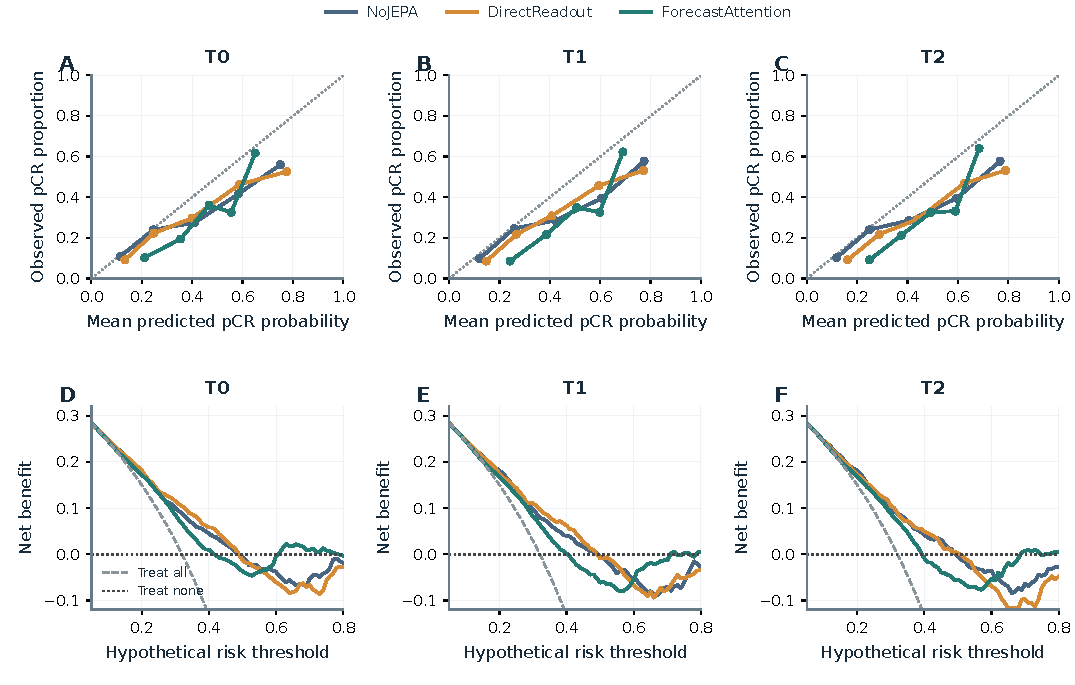
\includegraphics[width=\textwidth]{figures/calibration_utility.pdf}
\caption{Probability quality and hypothetical decision utility of separately evaluated fold models. (A--C) Reliability summaries form five equal-count probability-rank groups of 35 patients within each fold and then average the group summaries across folds; these differ from the ten equal-width bins used for ECE. (D--F) Net-benefit curves are computed per fold and averaged, with treat-all and treat-none references. Scores are not recalibrated or averaged between models. No clinical escalation or de-escalation strategy is validated.}
\label{fig:calutility}
\end{figure*}

\subsection{Hypothetical net benefit}
At a hypothetical threshold of 0.30, mean Macro net benefit was 0.1100 for \direct{} and 0.0850 for \fullmodel{}. At 0.50, all principal variants had negative mean Macro net benefit: $-0.0057$ for \nojepa{}, $-0.0069$ for \direct{}, and $-0.0510$ for \fullmodel{}. At 0.70, forecast attention had +0.0013, compared with $-0.0801$ for direct readout. The ordering therefore depended on threshold. These fold means use uncalibrated probabilities and a generic positive-action utility; they do not establish a clinical threshold or validate a management pathway.

\subsection{Exploratory biological and acquisition-related subgroups}
The full-versus-\nojepa{} mean Macro AUROC differences varied across HR/HER2 groups (Fig.~\ref{fig:subgroups}; Table~\ref{tab:subgroups}). They were +0.0324 [$-0.0153$, 0.0811] in HR-positive/HER2-negative patients (68 patients, 11 positive), $-0.0415$ [$-0.1353$, 0.0457] in HR-positive/HER2-positive patients (31, 12 positive), +0.0082 [$-0.1483$, 0.1483] in HR-negative/HER2-positive patients (14, 7 positive), and +0.0217 [$-0.0245$, 0.0667] in HR-negative/HER2-negative patients (62, 26 positive). Every interval included zero, and one subgroup's point estimate favored \nojepa{}. These unadjusted exploratory summaries do not establish a subtype-specific benefit or interaction.

In HR-positive/HER2-negative patients, forecast attention's mean Macro sensitivity/specificity was 0.2970/0.8713, compared with 0.0970/0.9696 for \nojepa{} and 0.1576/0.9591 for \direct{}. Greater sensitivity thus accompanied lower specificity in this group. Age and source-namespace summaries are descriptive; the namespaces share one clinical release and do not constitute external validation. The partially clipped baseline-component group contained 11 patients and only one positive outcome, so its AUROC and AP were suppressed under the minimum-outcome rule.

\begin{figure*}[t]
\centering
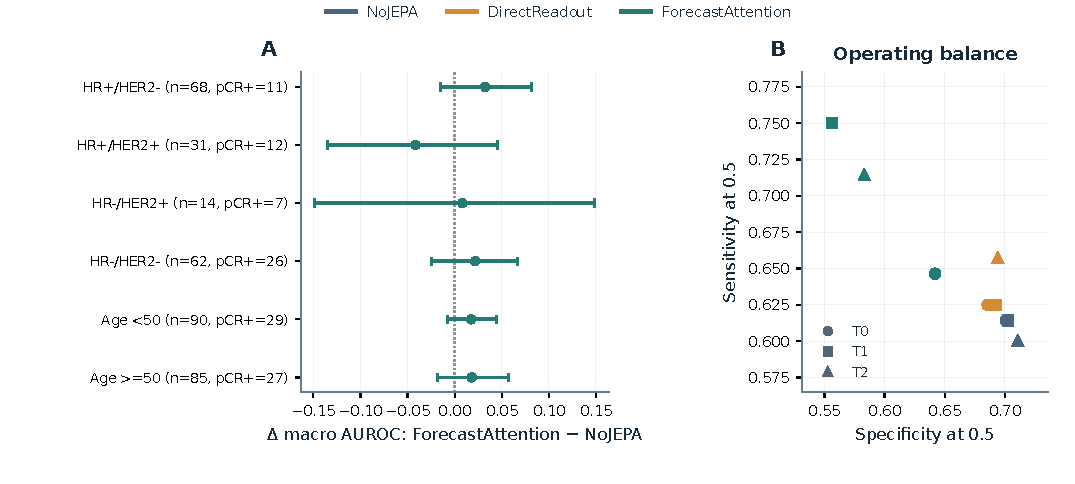
\includegraphics[width=\textwidth]{figures/subgroup_operating.pdf}
\caption{Exploratory subgroup and operating-point summaries, computed separately within seed-44 folds and averaged across folds. (A) Macro AUROC differences between ForecastAttention and NoJEPA within HR/HER2 and age groups, with patient counts, positive outcomes, and unadjusted shared-patient intervals. No subgroup-interaction claim is made. (B) Mean specificity and sensitivity at threshold 0.5 across landmarks; colors identify variants and markers identify landmarks.}
\label{fig:subgroups}
\end{figure*}

\subsection{Archived forecast and gradient diagnostics}
Archived fixed-training-probe diagnostics describe individual fold models separately from the pCR holdout analysis (Fig.~\ref{fig:mechanism}). At common epoch 20, mean copy-normalized forecast skills for \direct{} were +0.0258, +0.0500, and +0.1935 at one-, two-, and three-step horizons. Corresponding values for \fullmodel{} were $-0.0368$, $-0.0154$, and +0.0242 (Table~\ref{tab:worldprobe}). Statistics were normalized within each snapshot's EMA coordinates and averaged across the five seed-44 fold models. Latent states were not combined. These diagnostics do not support attributing forecast attention's ranking means to uniformly more accurate latent forecasts.

The probe requires the real landmark, target, and every intermediate examination, whereas the training objective masks unavailable future targets. Eligible populations therefore vary by horizon; only 5--9 patients per probe were eligible at three steps. These are not selected-checkpoint holdout forecast measurements. The predictor's pCR-loss gradient norm was zero for \direct{} and had mean 0.7148 for \fullmodel{}; weighted rollout-gradient means were 0.1213 and 0.1308. These values support the expected gradient routing, but gradient magnitude is not a biological effect size. \nojepa{} had no available trained-world diagnostic and was not assigned an artificial zero skill.

\begin{figure*}[t]
\centering
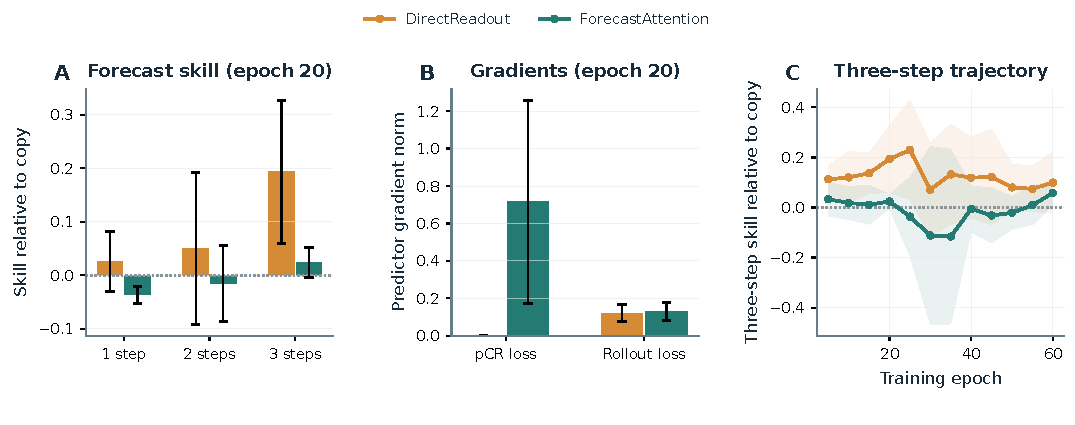
\includegraphics[width=\textwidth]{figures/forecast_mechanism.pdf}
\caption{Archived seed-44 fixed-training-probe diagnostics. (A) Copy-normalized forecast skill at common epoch 20. (B) Predictor gradient norms from pCR and weighted rollout losses. (C) Three-step skill across epochs with complete diagnostic coverage. Statistics are calculated within each snapshot's EMA coordinates and summarized descriptively across five folds. These training diagnostics are distinct from holdout pCR metrics; real continuous visit chains are required, and three-step eligibility is only 5--9 patients per probe.}
\label{fig:mechanism}
\end{figure*}
